\documentclass[english,serif,mathserif,xcolor=pdftex,dvipsnames,table]{beamer}

\usepackage[T1]{fontenc}
\usepackage[utf8]{inputenc}

\usetheme[informal]{s3it}
\usepackage{s3it}

\title[1. Basics]{%
  A Short and Incomplete Introduction to Python
}
\subtitle{\bfseries Part 1: Basic Python syntax}
\author[S.~Haug]{%
  \textbf{Sigve Haug} \texttt{<sigve.haug@math.unibe.ch>}, \\
  Alexander Kashev \texttt{<alexander.kashev@math.unibe.ch>} \\
  Science IT Support (ScITS), University of Bern \\
  \medskip
  Based on a course by Riccardo Murri / Sergio Maffioletti
  \\
  S3IT: Services and Support for Science IT, UZH
}
\date{August 20--21, 2018}


\begin{document}

% title frame
\maketitle

\part{Python basics}

\begin{frame}[fragile]
  \frametitle{Lines of Python code}
  Python code is interpreted line by line.

  \+
  A line is terminated simply by pressing "Enter".
  Python does not use semicolons or other separators.

  \+
  A long line can be split in two by ending it with the
  character `\texttt{\textbackslash}'; for example:
\begin{semiverbatim}
\In "hello" + \textbackslash
\Ct " world!"
\Out 'hello world!'
\end{semiverbatim}

  \+\scriptsize
  Reference:
  \url{http://docs.python.org/reference/lexical_analysis.html#line-structure}
\end{frame}


\begin{frame}[fragile]
  \frametitle{Comments}
  Anything following the pound sign `\#' is a comment
  and is not executed.

  \+
  It's used to leave notes to yourself or others in code,
  or temporarily disable parts of code.

\begin{semiverbatim}
# This is a comment
print("Hello, world!") # Basic example

# Code below won't be executed
# print("Goodbye, world!")
\end{semiverbatim}

  Writing good comments is important for understanding code later!
\end{frame}


\section{Variables, data types, and operations}

\begin{frame}[fragile]
  \frametitle{Data and basic types}

  Python can operate on different \textbf{types} of data,
  e.g. numbers, strings, booleans (true/false), lists of other data, etc.
  
  \+
  To add those to your code directly (as constants),
  you need \textbf{literals}.

  \+
  The next slides show examples for some basic types.
\end{frame}

\begin{frame}[fragile]
  \frametitle{Number literals}

  Python operates with \textbf{integers} and \textbf{floating point} numbers (floats).

  \+
  Integers in Python 3 can be arbitrarily large, while floating point numbers
  are subject to precision limits.
  
  \+
  A basic integer literal is just writted down as a number:
  
  \texttt{-1}, or \texttt{1234}, or \texttt{10000000000000000000}

  \+
  A number is understood as a floating point literal if it has a decimal dot in it:

  \texttt{3.1415}, or \texttt{10.0}, or even \texttt{1.} and \texttt{.005}

  \+\scriptsize
  Reference:
  \href{https://docs.python.org/3/library/stdtypes.html#numeric-types-int-float-complex}{Built-in Types: Numeric Types}
\end{frame}

\begin{frame}[fragile]
  \frametitle{String literals, I}
  Strings are the data type for text: sequences of individual characters.
  There are several ways to express string literals in Python.

  \+
  Single and double quotes can be used interchangeably to delimit strings:
\begin{semiverbatim}
"a string"
'a string'
\end{semiverbatim}
\end{frame}

\begin{frame}[fragile]
  \frametitle{String literals, II}

  You can use the single quotes inside double-quoted strings, and vice versa:
\begin{semiverbatim}
"Isn't it ok?"
'"Yes", he said.'
\end{semiverbatim}

  Or, you can use \textbf{escape sequences} to prevent quotes from ending the string:
  
  {
  \smaller
\begin{semiverbatim}
\In print("\\"It's unnecessarily complex,\\" he thought.")
\Out "It's unnecessarily complex," he thought.
\end{semiverbatim}
  }

Other useful escape sequences:

  \texttt{\textbackslash\textbackslash} for \textbackslash,
  \texttt{{\textbackslash}n} for a line break, \texttt{{\textbackslash}t} for a tab stop

\end{frame}


\begin{frame}[fragile]
  \frametitle{String literals, III}
  Multi-line strings are delimited by three quote characters.
\begin{lstlisting}[showstringspaces=false]
"""This is a string,
that extends over more
than one line.
"""
\end{lstlisting}

  You do not need not use the backslashes
  ``\texttt{\textbackslash}'' at the end of the lines
  to join them into one Python line.
\end{frame}


\begin{frame}[fragile]
  \frametitle{Operators, arithmetic}
  All the arithmetic operators are
  defined in Python:
  
  \texttt{+}, \texttt{-}, \texttt{*}, \texttt{/}, \texttt{**}~(exponentiation $x^y$), etc.

  \+
  Usually, the result of the operation is a float if at least one argument is.

  \+
  Python's division always produces a float.

  If you need integer division, you can use \texttt{//} for the result
  and \texttt{\%} for the remainder:

{
\smaller
\begin{semiverbatim}
\In 11 / 3
\Out 3.6666666666666665
\In 11 // 3
\Out 3
\In 11 % 3
\Out 2
\end{semiverbatim}
}
\end{frame}

\begin{frame}[fragile]
  \frametitle{Booleans and logic}

  Boolean (truth) values in Python are expressed using constants
  \texttt{True} and \texttt{False}.

  \+
  Logical operators are expressed using plain English words:
  \texttt{and}, \texttt{or}, \texttt{not}.

  \+
  Boolean values often come from numerical and string comparison:
  \texttt{<}, \texttt{>}, \texttt{<=}, \texttt{==}, \texttt{!=},
  \ldots

  \begin{references}
    \tiny
    \begin{itemize}
    \item
      \url{http://docs.python.org/library/stdtypes.html#boolean-operations-and-or-not}
    \item
      \url{http://docs.python.org/library/stdtypes.html#comparisons}
    \end{itemize}
  \end{references}
\end{frame}


\begin{frame}
  \frametitle{Your first exercise}
  %\href{http://www.pythonchallenge.com}{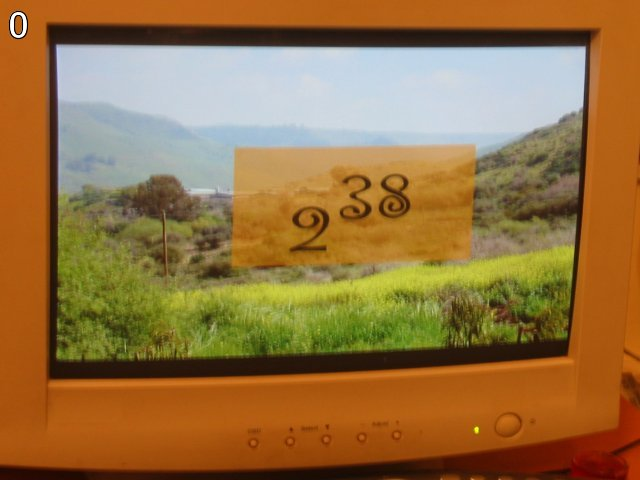
\includegraphics[width=\linewidth]{fig/2to38}}
    \begin{center}
      {\Large How much is \href{http://www.pythonchallenge.com}{$2^{144}$} ?}

      \+ (You have 1 minute time.)
    \end{center}
\end{frame}


\begin{frame}[fragile]
  \frametitle{Operators, II}
  \smaller

  Some operators are defined for non-numeric types:
\begin{lstlisting}
>>> "Py" + 'thon'
'Python'
\end{lstlisting}

  \+
  Some support operands of mixed type:
\begin{lstlisting}
>>> "a" * 2
'aa'
>>> 2 * "a"
'aa'
\end{lstlisting}

  \+
  Some do not:
\begin{lstlisting}[basicstyle=\footnotesize\ttfamily]
>>> "aaa" / 3
Traceback (most recent call last):
  File "<stdin>", line 1, in <module>
TypeError: unsupported operand type(s) for /: 'str' and 'int'
\end{lstlisting}
\end{frame}


\begin{frame}[fragile]
  \frametitle{Variables and assignment}

  You can't do much programming with just constants.
  To manipulate data, you need to store it somewhere.

  \+
  \textbf{Variables} are names for pieces of data in memory.

  \+
  Names must start with a letter, and can contain letters, numbers and underscores `\_'.

  \+
  You can assign \textbf{values} to them with the assignment operator \texttt{=},
  and use them in other expressions:

\begin{semiverbatim}
\In a = 11
\In b = 3
\In c = a - b
\In c
\Out 8
\end{semiverbatim}
\end{frame}


\begin{frame}[fragile]
  \frametitle{Assignment, II}
  Trying to use a variable that was never assigned produces an error.
  
  \+
  You can reassign values to already declared variables.

  Python is said to have \emph{loose typing:} a variable
    can point to any data, regardless of its type.

\begin{semiverbatim}
\In a = 11
\In a = "orange"
\In a = True
\end{semiverbatim}

  For binary operators, you can use assignment shortcuts,
  for example:

  \+
  \texttt{a = a + b} is the same as \texttt{a += b}.

\end{frame}


\begin{frame}[fragile]
  \frametitle{Best practice: variable naming}
  
  While it's fast to write shorter variable names,
    it's important to make your code easy to understand.

  \+
  Making longer but more meaningful names is recommended,
    especially if the variable is used in distant parts
    of the code. Compare:

\begin{semiverbatim}
\In a = w * h
\In area = width * height
\end{semiverbatim}

Which is easier to read?
\end{frame}


\begin{frame}[fragile]
  \frametitle{String interpolation}
  The \lstinline|.format()| method can be used to substitute values into placeholder
  strings.

  \+ \pause
  Placeholders can indicate substitutions by number (starting at 0):
\begin{lstlisting}[basicstyle=\footnotesize\ttfamily]
>>> "This is slide ~\alt<2>{\HL{\small\ttfamily\{0\}}}{\small\ttfamily\{0\}}~ of ~\alt<2>{\HL{\small\ttfamily\{1\}}}{\small\ttfamily\{1\}}~".format(20, 1001)
'This is slide 20 of 1001.'
\end{lstlisting}

  \+ \pause
  You can use names instead of numbers (then the order parameter occur in
  \lstinline|format()| does not matter):
\begin{lstlisting}[basicstyle=\footnotesize\ttfamily]
>>> "Today is ~\alt<3>{\HL{\small\ttfamily\{month\}}}{\{month\}}~ ~\alt<3>{\HL{\small\ttfamily\{day\}}}{\small\ttfamily\{day\}}~".format(day=2, month='March')
'Today is March 2'
\end{lstlisting}

  \begin{references}
    \url{https://pyformat.info/}
  \end{references}
\end{frame}

\begin{frame}[fragile]
  \frametitle{Exercise}

  \begin{exercise*}[1.B]

    Save your weight (in kg) and height (in m) into variables.

    Calculate your BMI and save it into a variable.

    \+
    Hint: $\mathsf{bmi} = \frac{\mathsf{weight}}{\mathsf{height}^2}$

    \+
    Use \texttt{.format()} to display "My BMI is <number>"
  \end{exercise*}
\end{frame}

\begin{frame}[fragile]
  \frametitle{Basic types}
  Basic object types in Python 3:
  \begin{description}
  \item[None] Special type with one value \texttt{None}.
  \item[bool] Truth values: \texttt{True}, \texttt{False}.
  \item[int] Integer numbers: \texttt{1}, \texttt{-2}, \ldots
  %   up to \texttt{9223372036854775807} (on a 64-bit machine)
  % \item[long] Integer numbers of arbitrary size; Python switches
  %   automatically from \texttt{int} to \texttt{long} when needed.
  \item[float] Double precision floating-point numbers, e.g.:
    \texttt{3.1415}, \texttt{-1e-3}.
  \item[bytes] String of byte-size characters.
  \item[str] Text (string of UNICODE characters).
  %\item[unicode] Strings of UNICODE characters.
  \item[list] Mutable list of Python objects
  \item[dict] Key/value mapping
  \end{description}

  \+ The type of a Python object can be gotten via the \texttt{type()} function:
\begin{semiverbatim}
{\color{blue}\bfseries In [3]:} type('hello')
{\color{red}\bfseries Out[3]:} str
\end{semiverbatim}
\end{frame}

\end{document}

%%% Local Variables:
%%% mode: latex
%%% TeX-master: t
%%% End:
